\chapter{Introduction} 
\label{chapter:introduction}



%\begin{figure}[!h]
%\captionsetup{format=hang}
%\centering
%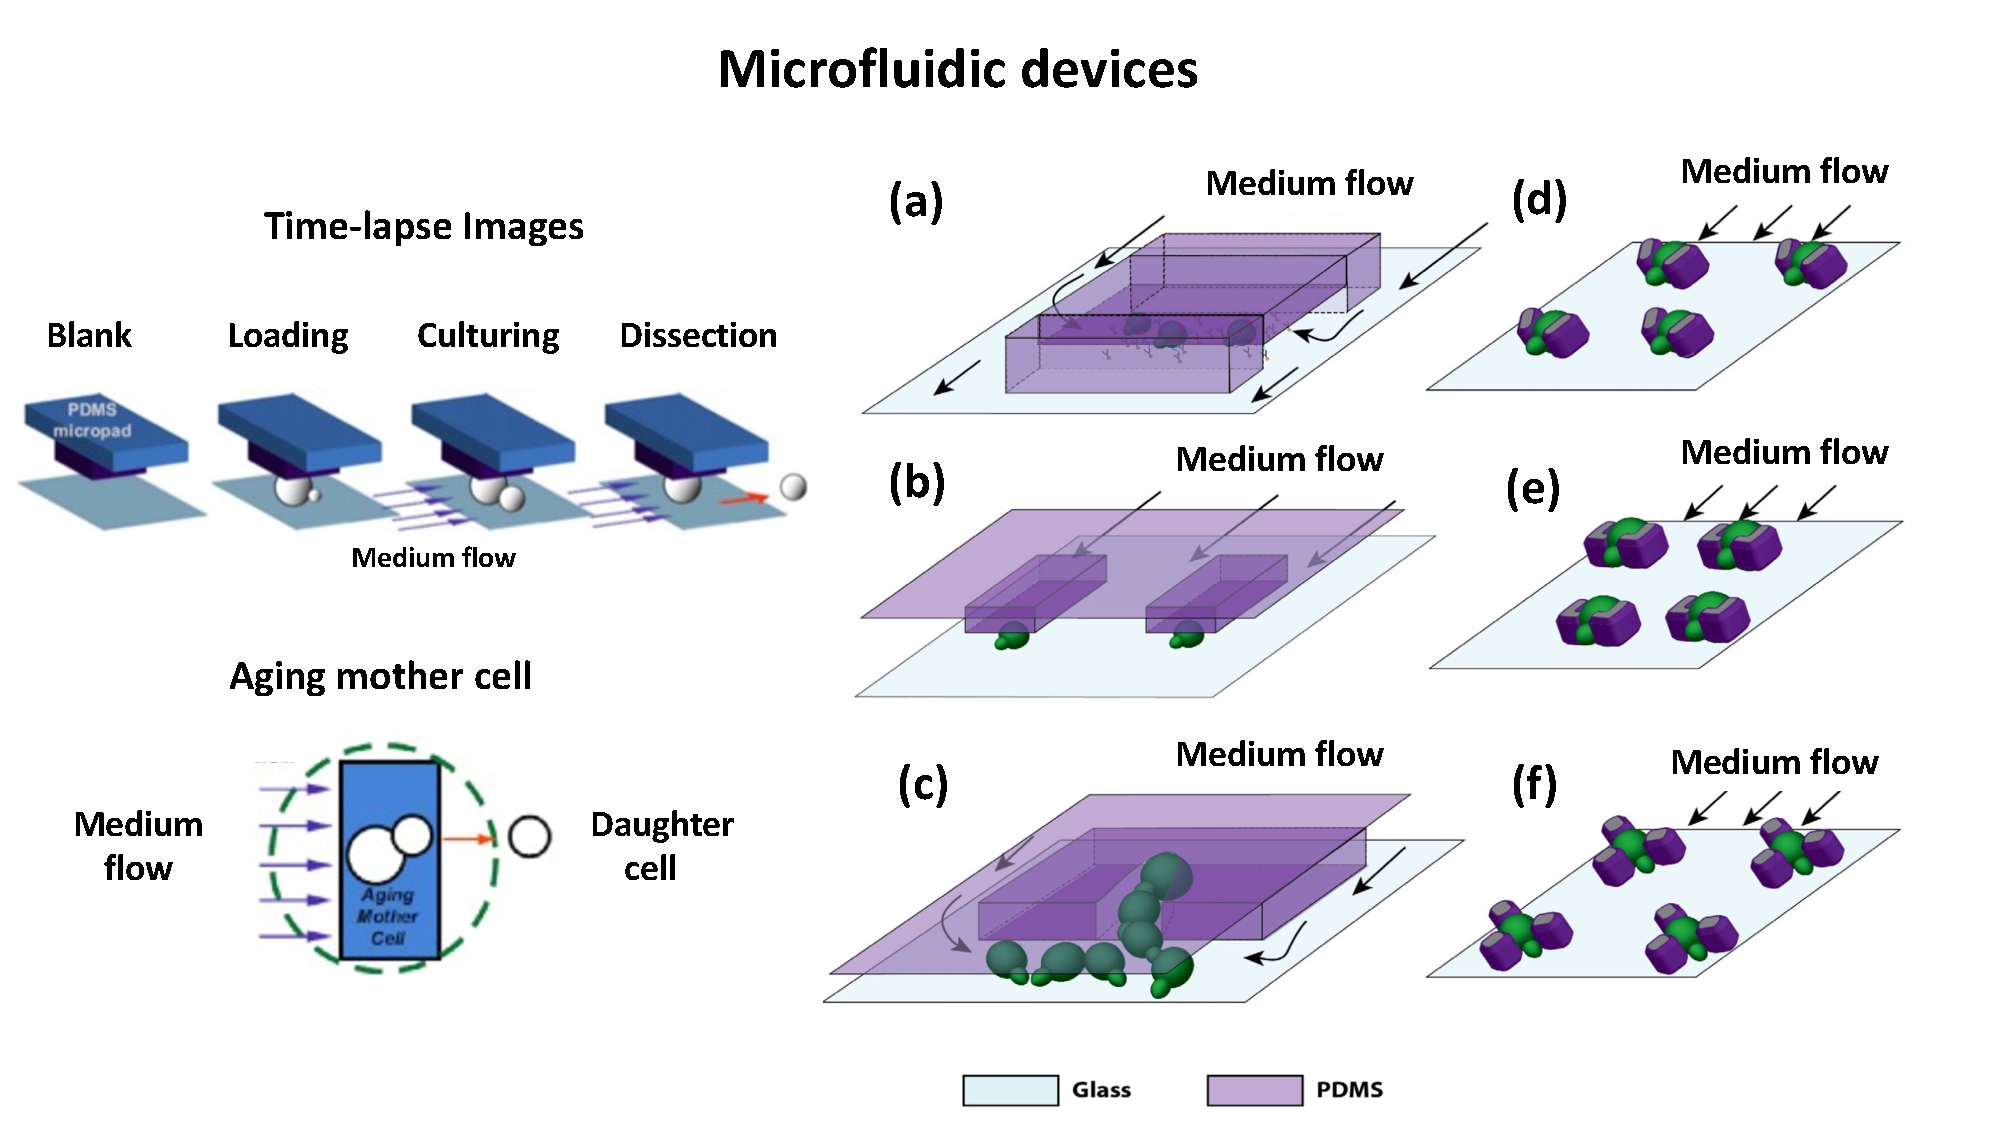
\includegraphics[width=1\textwidth,height=0.5\textheight,angle %=0]{dissertation/figures/data/microfludic.pdf}
%\caption{ The generic type of microfluidic devices. Patterns a, b and c %are considered as low-throughput. Patterns d, e, and f are considered as %high-throughput}
%\label{fig:micro}
%\end{figure} 


\section{Outline}

%The remainder of this dissertation is organized as follows. Chapter \ref{microfluidic} provides background and review of relevant literature surrounding segmentation methods and model comparison. Chapter \ref{classify} provides some information on microfluidic devices, time series microfluidic images and steps for data collection. Chapter \ref{Mask_yolo} covers deep learning model comparison for microfluidic image classification with a suggesting model for better classification. Chapter \ref{tree} introduces an algorithm to generate a cell family tree from a feature extraction dataset and produce ID for an individual cell. Chapter \ref{upolar} introduces a visualization tool based on the R package. It visualizes time series microscopic images in 2D interactively. Chapter \ref{work} discusses the future works, and the conclusion of the work covers in chapter \ref{conclusion}.